\documentclass[10pt,a4paper]{article}
\usepackage[left=2cm,right=2cm,top=2cm,bottom=2cm]{geometry}
\usepackage[T1]{fontenc}
\usepackage{lmodern}
\usepackage[spanish,es-tabla,es-noquoting]{babel}
\usepackage[dvipsnames]{xcolor}
\usepackage[fleqn]{mathtools}
\usepackage{booktabs}
\usepackage{amsmath}
\usepackage{latexsym}
\usepackage{graphicx}
\usepackage{nccmath}
\usepackage{multicol}
\usepackage{listings}
\usepackage{tasks}
\usepackage{color}
\usepackage{float}
\usepackage{tikz}
\usepackage{csquotes}
\usepackage[backend=biber,style=numeric,sorting=none]{biblatex}
\addbibresource{referencias.bib}

\definecolor{colorIPN}{rgb}{0.5, 0.0,0.13}
\definecolor{colorESCOM}{rgb}{0.0, 0.5,1.0}
\graphicspath{ {imagenes/} }

\begin{document}
%#########################################################
\begin{titlepage}
	\centering
	{ \huge \bfseries \color{colorIPN}{Instituto Politécnico Nacional} \par}
	{ \Large \bfseries  \color{colorESCOM}{Escuela Superior de Cómputo} \par }
	\vspace{1cm}
	{\huge\Large \color{colorIPN}{Web Client and Backend Development Frameworks}.\par}
	\vspace{1.5cm}
	{\huge\Large  \color{colorESCOM}{Descarga, creación y ejecución de imagen Docker del minisitio de nuevo ingreso de ESCOM}\par}
		\vspace{2cm}
	{\Large\itshape \color{colorIPN}{Profesor: Dr. José Asunción Enríquez Zárate}\par} \hfill \break
	\vspace{2cm}
	{\Large\itshape \color{colorIPN}{Alumno: Angel Frausto Robles}\par} \hfill \break
	{\Large\itshape \color{colorIPN}{Boleta: 2019630177}\par} \hfill \break
	{\Large\itshape \color{colorIPN}{id634296@gmail.com}\par} \hfill \break
	{\Large\itshape \color{colorIPN}{7CM2} \par}
	\vfill
	{\large \color{colorIPN}{\today}\par}
	\vfill
\end{titlepage}

\renewcommand\lstlistingname{Código}

\lstset{
	basicstyle=\small\sffamily,
	numbers=left,
	numberstyle=\tiny,
	frame=tb,
	tabsize=4,
	columns=fixed,
	showstringspaces=false,
	showtabs=false,
	keepspaces,
	commentstyle=\color{Violet},
	keywordstyle=\color{colorIPN} \bfseries,
	stringstyle=\color{colorESCOM},
	extendedchars=true,
	inputencoding=utf8,
	literate=
		{á}{{\'a}}1 {é}{{\'e}}1 {í}{{\'i}}1 {ó}{{\'o}}1 {ú}{{\'u}}1
		{Á}{{\'A}}1 {É}{{\'E}}1 {Í}{{\'I}}1 {Ó}{{\'O}}1 {Ú}{{\'U}}1
		{ñ}{{\~n}}1 {Ñ}{{\~N}}1 {ü}{{\"u}}1 {¿}{{?`}}1 {¡}{{!`}}1
}

\settasks{
	counter-format=(tsk[r]),
	label-width=4ex
}
\tableofcontents
\pagebreak
\listoffigures
\pagebreak
\listoftables
\pagenumbering {arabic}

\pagebreak

%################################################
\section{\color{colorIPN}{Introducción}}

Esta práctica retoma el minisitio de nuevo ingreso de ESCOM, ya descargado como copia fiel de \url{https://www.escom.ipn.mx/nuevoingreso27_1/} en una práctica anterior del curso, y lo usa como caso de estudio para publicar un sitio estático mediante Docker. El objetivo no es el sitio en sí, sino el mecanismo: empaquetar el mismo contenido dentro de dos imágenes distintas, una basada en Apache y otra en Nginx, y comprobar que ambos servidores lo sirven de forma idéntica desde el punto de vista del navegador.

Docker resuelve un problema concreto de despliegue: que un servicio corra igual en la máquina de desarrollo, en la de un compañero de equipo y en el servidor de producción, sin depender de qué versión de Apache o de Nginx tenga instalada cada máquina. Este reporte documenta el proceso completo, desde el contenido ya descargado hasta los dos contenedores corriendo en paralelo, con evidencia de cada comando y del resultado final en el navegador.

%################################################
\section{\color{colorIPN}{Conceptos teóricos}}

\subsection{ \color{colorESCOM}{Imagen Docker}}

Una imagen es una plantilla de solo lectura que contiene un sistema de archivos mínimo y las instrucciones necesarias para ejecutar una aplicación: el sistema operativo base, las dependencias y los archivos propios del proyecto \cite{docker2024overview}. Se construye una sola vez a partir de un Dockerfile y, a partir de ahí, es inmutable: para cambiar algo hay que reconstruirla, no modificarla en caliente. Cada instrucción del Dockerfile agrega una capa a la imagen, y Docker reutiliza las capas que no cambiaron entre una construcción y la siguiente.

\subsection{ \color{colorESCOM}{Contenedor}}

Un contenedor es una instancia en ejecución de una imagen, con una capa de escritura efímera encima de las capas de solo lectura de esa imagen \cite{docker2024overview}. A diferencia de una máquina virtual, no incluye su propio kernel: se aísla del sistema anfitrión y de otros contenedores mediante los \textit{namespaces} y los \textit{cgroups} del kernel de Linux, pero en tiempo de ejecución comparte ese kernel con el host. Esa diferencia es lo que hace que un contenedor arranque en fracciones de segundo en vez de en el tiempo que toma arrancar un sistema operativo completo. De una misma imagen pueden crearse tantos contenedores como se necesiten, cada uno con su propio estado y ciclo de vida.

\subsection{ \color{colorESCOM}{Dockerfile}}

El Dockerfile es un archivo de texto plano con instrucciones secuenciales que describen cómo construir una imagen \cite{docker2024dockerfile}. Instrucciones como \texttt{FROM}, \texttt{COPY}, \texttt{RUN} o \texttt{EXPOSE} se ejecutan en orden, y cada una produce una capa nueva sobre la anterior. Para un sitio completamente estático, como el de esta práctica, el Dockerfile puede ser mínimo: basta con partir de una imagen que ya trae el servidor web instalado y copiar los archivos del sitio a la carpeta que ese servidor sirve por defecto.

\subsection{ \color{colorESCOM}{Mapeo de puertos}}

Un contenedor corre en su propia red virtual y, aunque su proceso interno escuche en un puerto, ese puerto no es alcanzable desde el host a menos que se publique explícitamente \cite{docker2024ports}. La bandera \texttt{-p host:contenedor} de \texttt{docker run} le indica a Docker que reenvíe el tráfico que llega a un puerto del host hacia el puerto correspondiente dentro del contenedor. Esto es lo que permite correr dos contenedores que internamente usan el mismo puerto 80, uno servido con Apache y otro con Nginx, y aun así distinguirlos desde el navegador mediante dos puertos distintos del host.

%################################################
\section{\color{colorIPN}{Desarrollo}}

\subsection{ \color{colorESCOM}{Descarga del sitio}}

\begin{figure}[H]
	\centering
	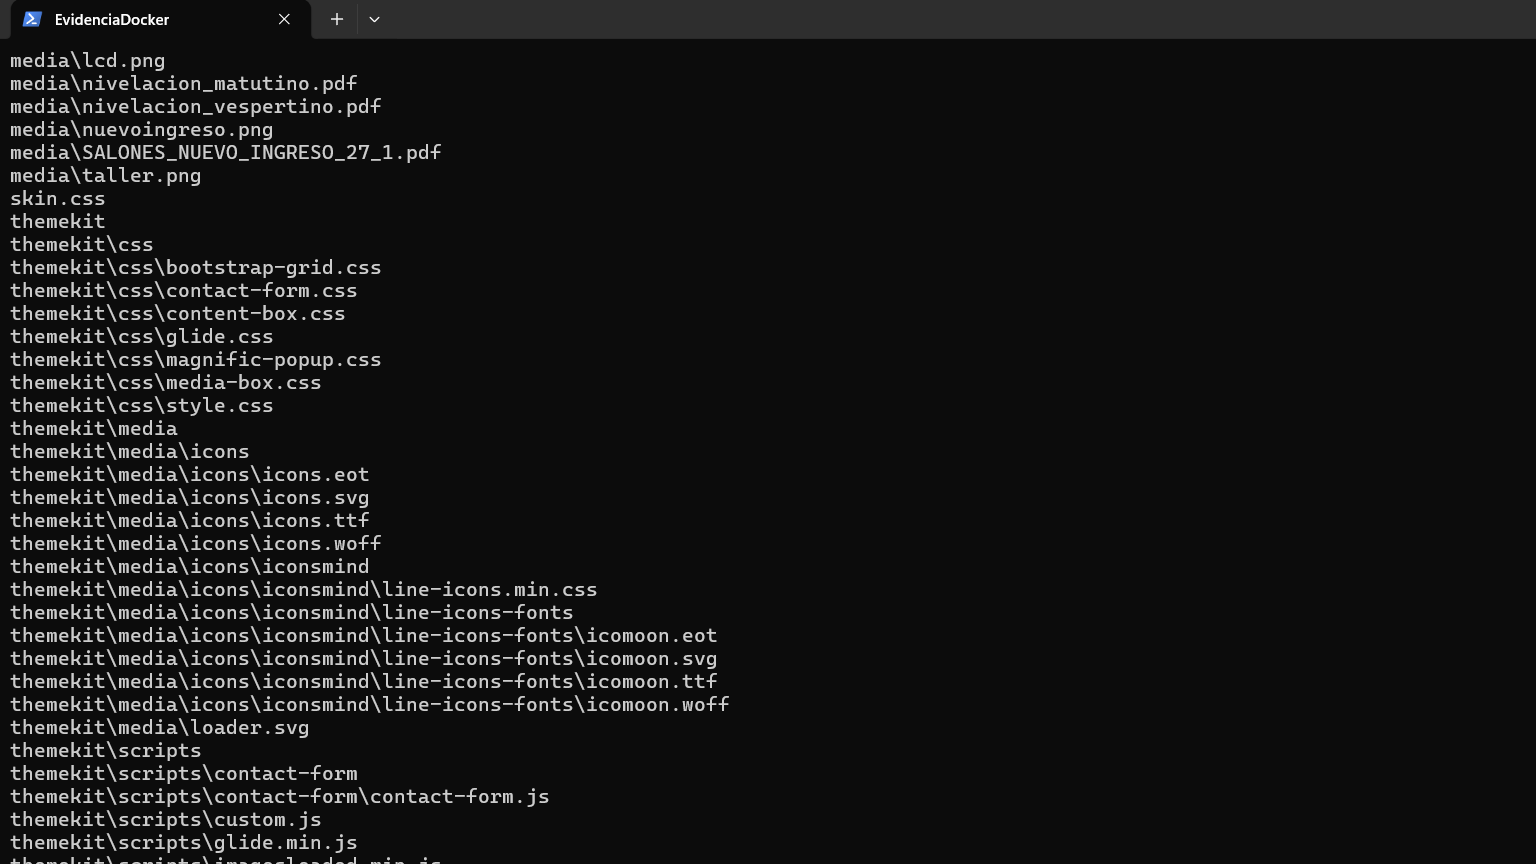
\includegraphics[width=0.9\textwidth]{captura1-descarga.png}
	\caption{Contenido del minisitio ya descargado, listo para servirse en ambas imágenes}
	\label{img:descarga}
\end{figure}

El contenido del minisitio ya estaba descargado de una práctica anterior del curso, que replicó \url{https://www.escom.ipn.mx/nuevoingreso27_1/} archivo por archivo. La figura \ref{img:descarga} muestra esa descarga: \texttt{index.html}, \texttt{skin.css} y la carpeta \texttt{themekit} con los estilos, íconos y scripts del tema, además de \texttt{media} con las imágenes y los PDF de asignación que el sitio original expone. Para esta práctica ese contenido se reutilizó como una única carpeta \texttt{sitio/}, compartida como contexto de construcción entre las dos imágenes, en vez de duplicar los mismos archivos dentro de cada una.

\subsection{ \color{colorESCOM}{Dockerfile de Apache}}

\begin{lstlisting}[language=bash,caption={Dockerfile.apache}, label={lst:dockerfileapache}]
FROM httpd:2.4-alpine
COPY . /usr/local/apache2/htdocs/
EXPOSE 80
\end{lstlisting}

\begin{itemize}
	\item \texttt{FROM httpd:2.4-alpine} parte de la imagen oficial de Apache httpd 2.4 sobre Alpine Linux \cite{apache2024docker}, una base minimalista que reduce el tamaño final de la imagen frente a una distribución completa.
	\item \texttt{COPY . /usr/local/apache2/htdocs/} copia todo el contexto de construcción, es decir, el contenido de \texttt{sitio/}, al \textit{DocumentRoot} que esa imagen sirve por defecto.
	\item \texttt{EXPOSE 80} documenta que el proceso de Apache dentro del contenedor escucha en el puerto 80. Por sí sola no publica nada hacia el host, eso lo hace \texttt{docker run -p}.
\end{itemize}

\subsection{ \color{colorESCOM}{Dockerfile de Nginx}}

\begin{lstlisting}[language=bash,caption={Dockerfile.nginx}, label={lst:dockerfilenginx}]
FROM nginx:alpine
COPY . /usr/share/nginx/html/
EXPOSE 80
\end{lstlisting}

La estructura es la misma que la del Dockerfile de Apache; solo cambian la imagen base y la carpeta de destino del \texttt{COPY}, que en la imagen oficial de Nginx es \texttt{/usr/share/nginx/html/} en vez de \texttt{/usr/local/apache2/htdocs/} \cite{nginx2024docker}. La tabla \ref{tabla:dockerfiles} resume esa diferencia.

\begin{table}[H]
	\centering
	\begin{tabular}{p{3cm} | p{5cm} | p{5cm}}\hline \hline
		& \textbf{Apache} & \textbf{Nginx} \\ \hline \hline
		Imagen base & \texttt{httpd:2.4-alpine} & \texttt{nginx:alpine} \\ \hline
		Carpeta de destino & \texttt{/usr/local/apache2/htdocs/} & \texttt{/usr/share/nginx/html/} \\ \hline
		Puerto interno & 80 & 80 \\ \hline
		Puerto publicado & 8080 & 8081 \\ \hline \hline
	\end{tabular}
	\caption{Diferencias entre los dos Dockerfile del mismo sitio}
	\label{tabla:dockerfiles}
\end{table}

\subsection{ \color{colorESCOM}{Construcción de las imágenes}}

\begin{figure}[H]
	\centering
	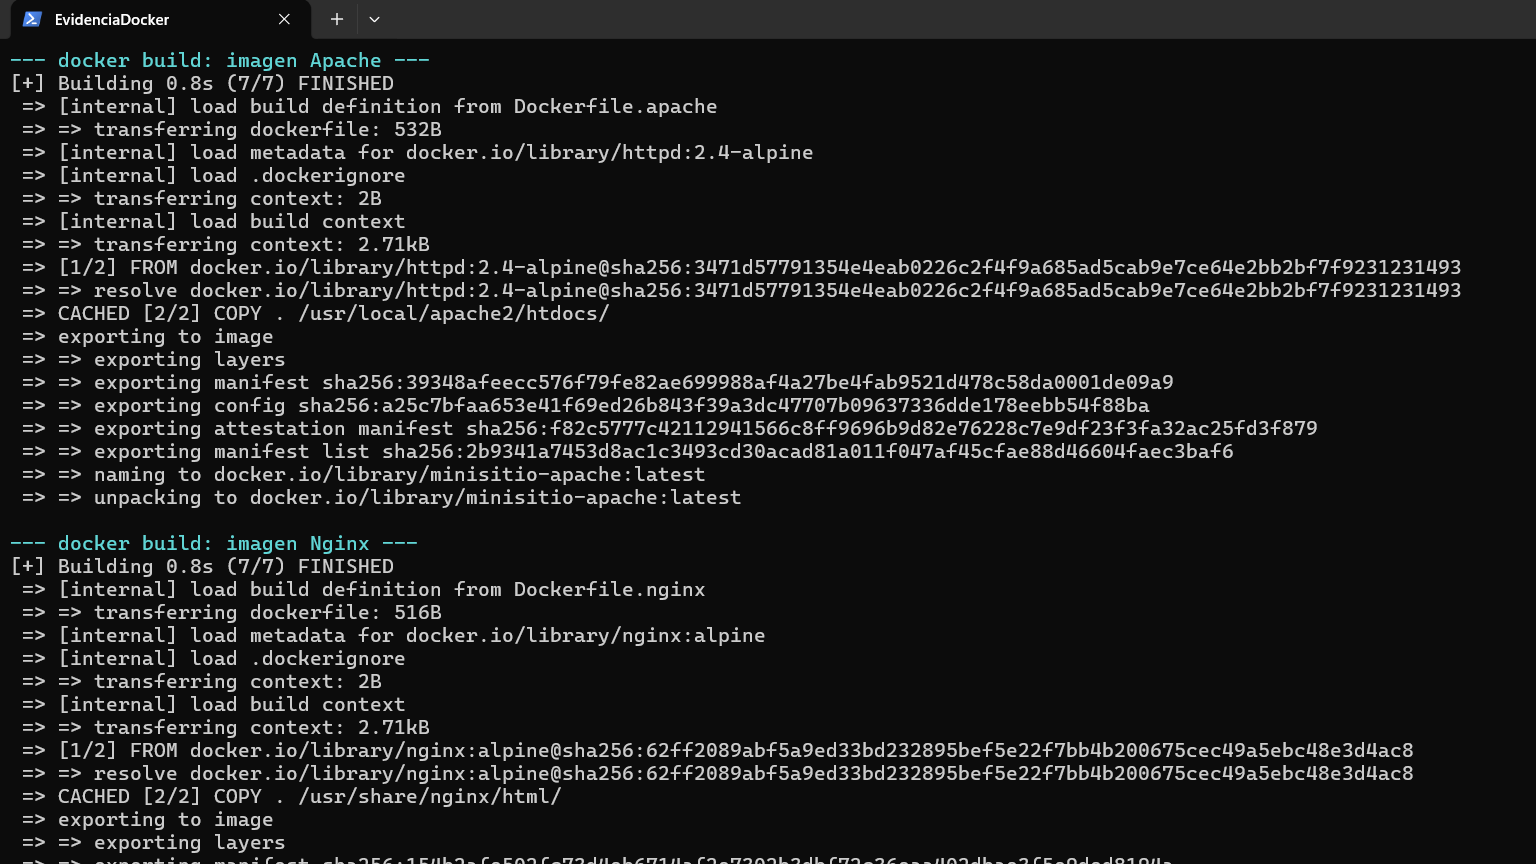
\includegraphics[width=0.95\textwidth]{captura2-build.png}
	\caption{docker build de las dos imágenes a partir del mismo contexto sitio/}
	\label{img:build}
\end{figure}

\begin{lstlisting}[language=bash,caption={Comandos de construcción}]
docker build -f Dockerfile.apache -t minisitio-apache ./sitio
docker build -f Dockerfile.nginx  -t minisitio-nginx  ./sitio
\end{lstlisting}

Como ninguno de los dos archivos se llama \texttt{Dockerfile} a secas, la bandera \texttt{-f} es obligatoria para indicar cuál usar en cada construcción. La bandera \texttt{-t} etiqueta la imagen resultante con un nombre legible, y \texttt{./sitio} es el contexto de construcción: la carpeta cuyo contenido se envía al daemon de Docker y queda disponible para las instrucciones \texttt{COPY} del Dockerfile. La figura \ref{img:build} muestra las dos construcciones completas, cada una con sus siete pasos internos (carga del Dockerfile, resolución de la imagen base, transferencia del contexto, copia de archivos y exportación de la imagen final) terminando en \texttt{naming to docker.io/library/minisitio-apache:latest} y su equivalente para Nginx.

\subsection{ \color{colorESCOM}{Ejecución de los contenedores}}

\begin{figure}[H]
	\centering
	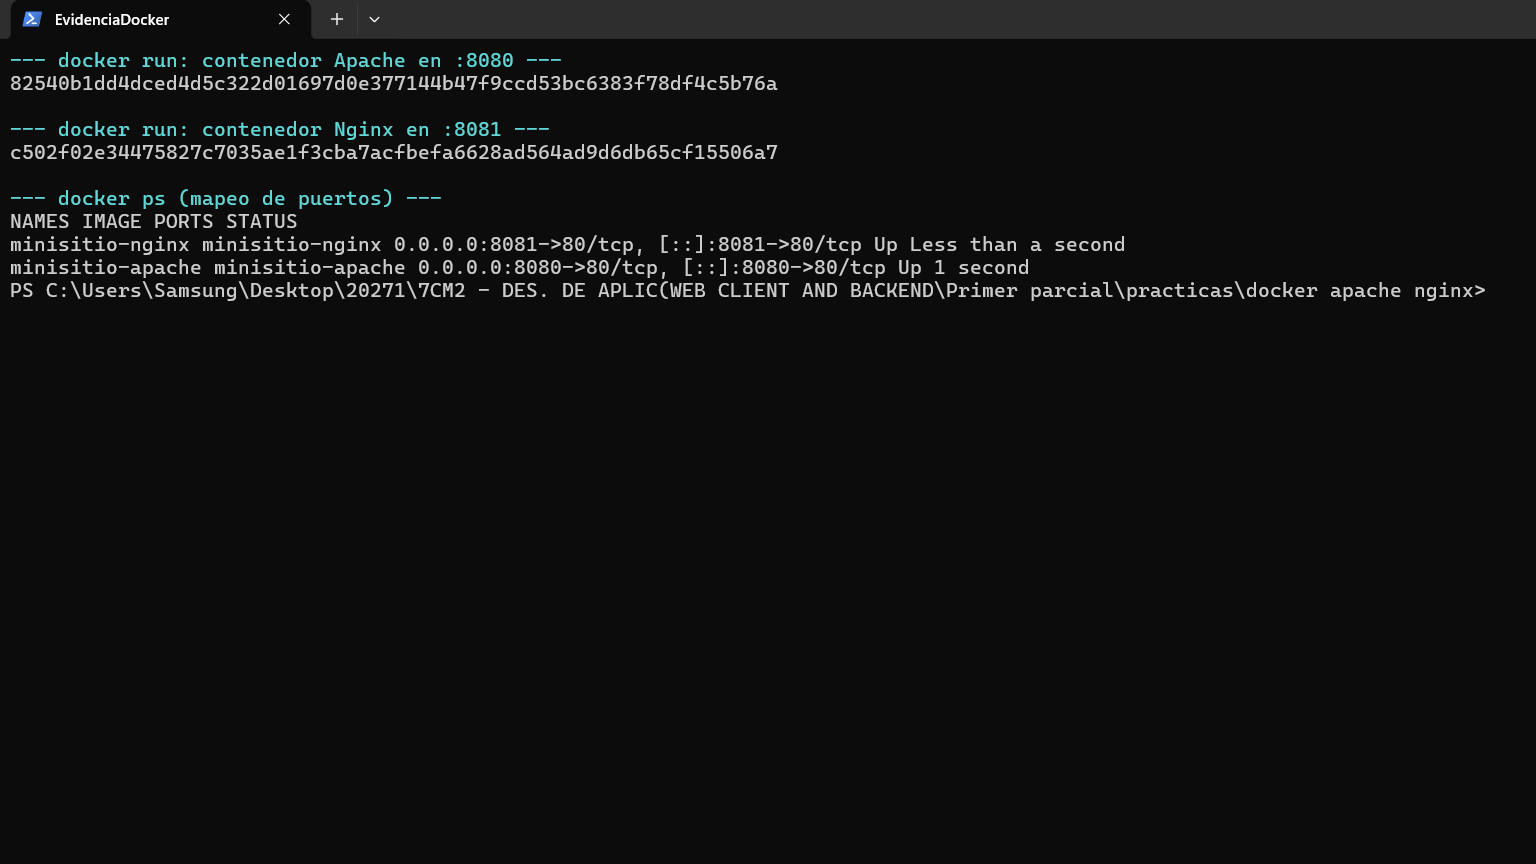
\includegraphics[width=0.95\textwidth]{captura3-run.png}
	\caption{docker run de ambos contenedores y verificación del mapeo de puertos con docker ps}
	\label{img:run}
\end{figure}

\begin{lstlisting}[language=bash,caption={Comandos de ejecución}]
docker run --name minisitio-apache -dit -p 8080:80 minisitio-apache
docker run --name minisitio-nginx  -dit -p 8081:80 minisitio-nginx
\end{lstlisting}

\texttt{--name} asigna un nombre legible al contenedor en vez de dejarlo con uno generado al azar. \texttt{-d} lo corre en segundo plano, \texttt{-i} mantiene abierta la entrada estándar y \texttt{-t} le asigna una pseudo-terminal; la combinación \texttt{-dit} es una convención común aunque, para un servidor web puramente estático como este, el contenedor no necesita interactividad para funcionar. La parte que sí es indispensable es \texttt{-p 8080:80} y \texttt{-p 8081:80}: publican el puerto 80 interno de cada contenedor en dos puertos distintos del host, para poder distinguir ambos servidores desde el navegador. La figura \ref{img:run} confirma, con \texttt{docker ps}, que los dos contenedores quedaron arriba (\textit{Up}) y con el mapeo de puertos esperado.

%################################################
\section{\color{colorIPN}{Resultados}}

\subsection{ \color{colorESCOM}{Verificación en el navegador}}

\begin{figure}[H]
	\centering
	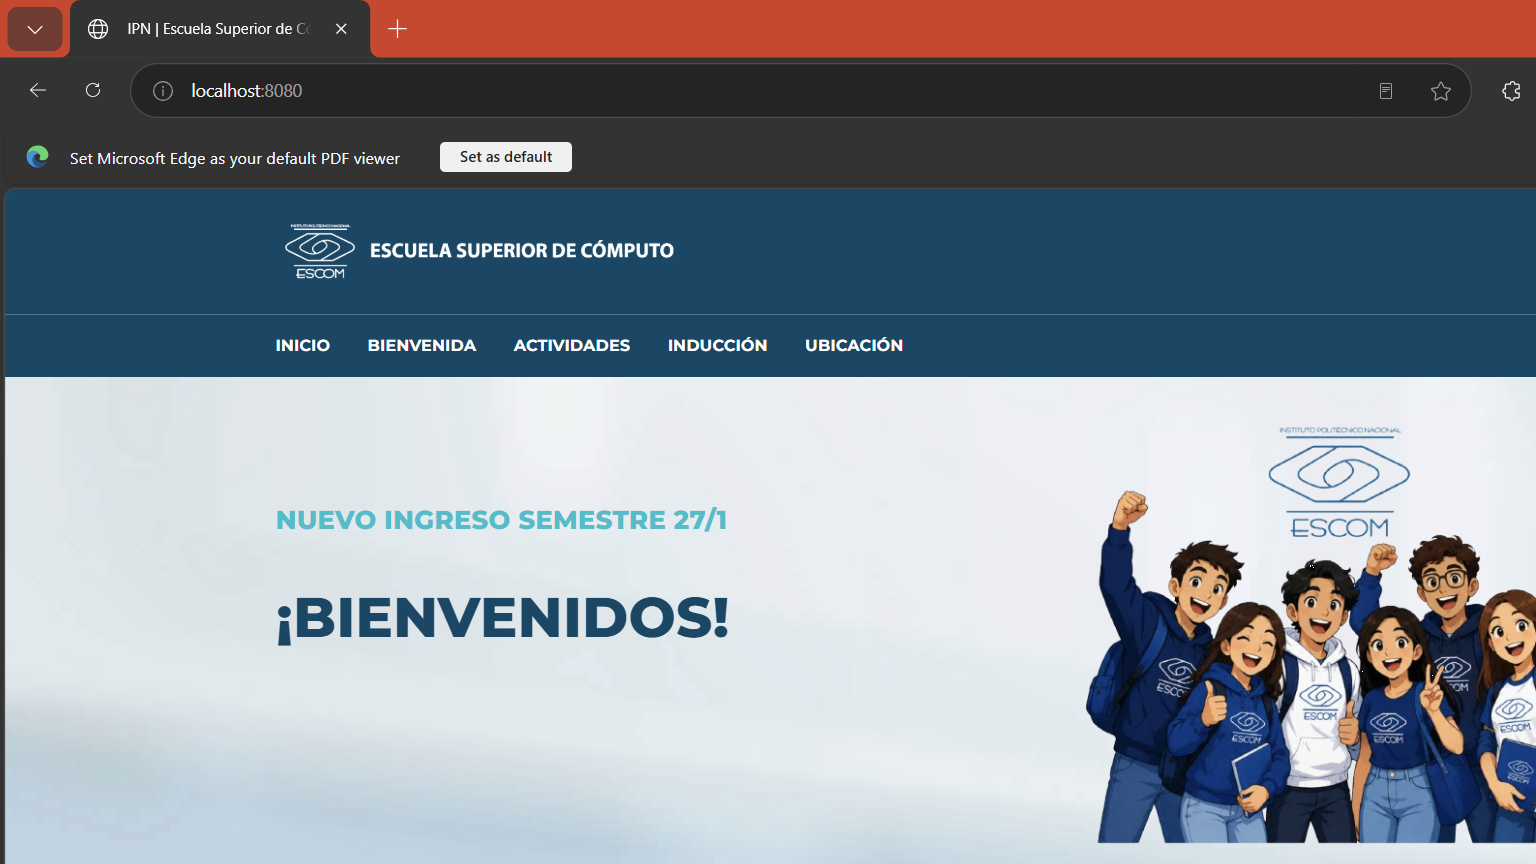
\includegraphics[width=0.95\textwidth]{captura4-navegador-8080.png}
	\caption{Minisitio servido por el contenedor de Apache en http://localhost:8080}
	\label{img:nav8080}
\end{figure}

\begin{figure}[H]
	\centering
	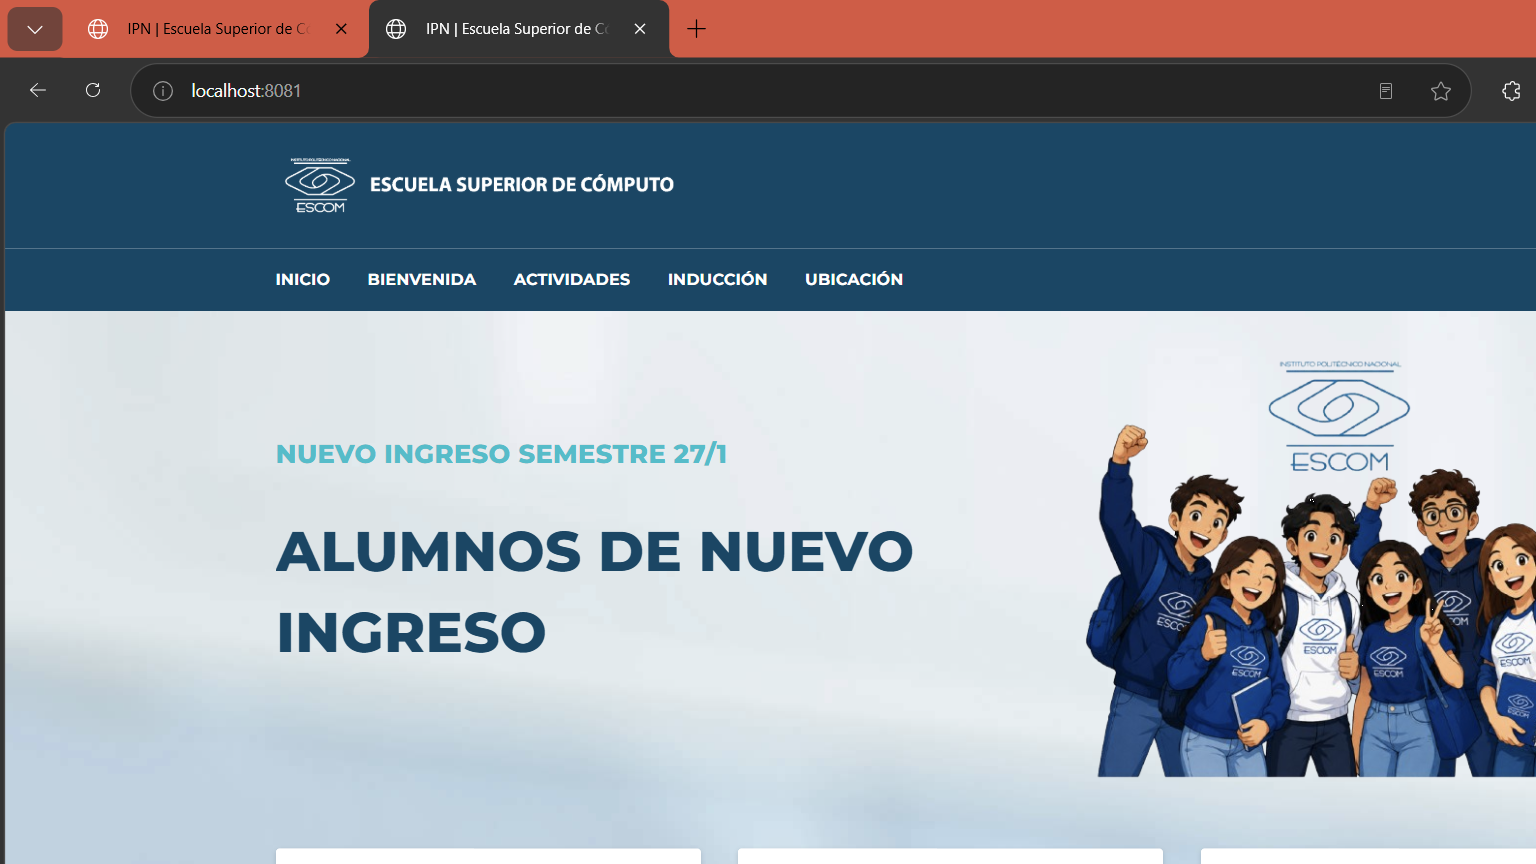
\includegraphics[width=0.95\textwidth]{captura5-navegador-8081.png}
	\caption{Minisitio servido por el contenedor de Nginx en http://localhost:8081, con el primero seguir abierto en la otra pestaña}
	\label{img:nav8081}
\end{figure}

Las figuras \ref{img:nav8080} y \ref{img:nav8081} muestran el mismo minisitio respondiendo en los dos puertos, con la barra de direcciones visible en cada caso. El contenido, los estilos y las imágenes se ven idénticos en ambas capturas porque provienen exactamente del mismo contexto de construcción; lo único que cambió fue el servidor web que lo entrega.

\subsection{ \color{colorESCOM}{Resumen de resultados}}

\begin{table}[H]
	\centering
	\begin{tabular}{p{3cm} | p{3.5cm} | p{2.5cm} | p{3cm}}\hline \hline
		\textbf{Servidor} & \textbf{Imagen base} & \textbf{Puerto host} & \textbf{Respuesta HTTP} \\ \hline \hline
		Apache httpd & httpd:2.4-alpine & 8080 & 200 OK \\ \hline
		Nginx & nginx:alpine & 8081 & 200 OK \\ \hline \hline
	\end{tabular}
	\caption{Estado final de los dos contenedores}
	\label{tabla:resultados}
\end{table}

Ambos contenedores respondieron con código 200 al pedir la raíz del sitio, lo que confirma que el \textit{DocumentRoot} quedó bien copiado en los dos casos y que el mapeo de puertos funciona en ambas direcciones.

%################################################
\section{\color{colorIPN}{Conclusiones}}

La práctica deja clara la diferencia entre imagen y contenedor de una forma que la definición por sí sola no transmite: la misma imagen \texttt{minisitio-apache} se pudo detener, eliminar y volver a correr con \texttt{docker run} sin reconstruirla, porque la imagen es la plantilla fija y el contenedor es la instancia desechable que se crea a partir de ella. También quedó claro que, para un sitio puramente estático, el Dockerfile no necesita más de tres instrucciones: la complejidad de un proyecto Docker está casi siempre en la aplicación que corre adentro, no en el mecanismo de empaquetado en sí.

El Dockerfile no dio ningún problema; lo complicado fue el entorno. El primer intento de \texttt{docker build} falló porque el daemon de Docker no estaba corriendo (\textit{failed to connect to the docker API... check if the path is correct and if the daemon is running}), ya que Docker Desktop no se había iniciado en la sesión. Se resolvió iniciando Docker Desktop manualmente y esperando a que el motor terminara de levantar antes de reintentar. La otra decisión que tomó tiempo fue evitar duplicar dos veces los mismos catorce megabytes de recursos del sitio: en vez de copiar el contenido dentro de cada Dockerfile, se dejó una sola carpeta \texttt{sitio/} compartida como contexto de construcción entre ambas imágenes, usando la bandera \texttt{-f} para apuntar a cada Dockerfile por separado.

%################################################
\pagebreak

\section{\color{colorIPN}{Referencias Bibliográficas}}
\color{colorESCOM}{
	\printbibliography[heading=none]
}

\end{document}
